\documentclass[a4peper, 12pt, twoside]{report}
\usepackage[utf8]{inputenc}
\usepackage[T1]{fontenc}
\usepackage[italian]{babel}
\usepackage{amsmath}
\usepackage{amssymb}
\usepackage{titlesec}
\usepackage{multicol}
\usepackage{xcolor}
\usepackage{tikz}
\usetikzlibrary{angles,quotes}
\usepackage{graphicx}

% Emphasis as bfseries
\DeclareEmphSequence{\bfseries}
% Custom template UniVR
\usepackage{noteTemplate}
\newcommand{\CourseTitle}{Fisica II}
\newcommand{\Author}{Iselle Niccol\`o}
\newcommand{\Prof}{Daffara Claudia}
\newcommand{\AY}{2023 - 2024}

\graphicspath{ {./img/} }

\definecolor{shadecolor}{RGB}{210,210,210}
\newcommand{\defbox}[1]{\noindent\colorbox{shadecolor}
{\parbox{\dimexpr\textwidth-2\fboxsep\relax}{#1}}}

\titleformat{\chapter}
	{\Large\bfseries}		% format
	{}					% label
	{0pt}				% sep
	{\huge}				% before-code

% Authors email
\newcommand{\email}{niccolo.iselle@studenti.univr.it}

\begin{document}
\begin{titlepage}
    \centering
    \textsc{Universit\`a degli studi di Verona}
    \par\vspace{0.5cm}
    \rmfamily
    Dipartimento di informatica \\
    \AY
    \par\vspace{1cm}
    
\includegraphics[scale=0.5]{univr.png}
    \par\vspace{2cm}
    
    \textbf{\Huge{\underline{\CourseTitle}}}
    \par\vspace{0.5cm}
    
    \par\vspace{1cm}
    \footnotesize
    Corso tenuto da \\
    \normalsize
    \textsc{\Prof}
    \par\vspace{1cm}
    \footnotesize
    Appunti a cura di \\
    \normalsize
    \textsc{Iselle Niccol\`o}
    \par\vspace{1cm}
    
    \vfill
    \footnotesize
    Made with \LaTeX \\
    \small
    Comunicare eventuali refusi o errori a: \email.
\end{titlepage}
\afterpage{\blankpage}
\tableofcontents

\chapter{Forza elettromagnetica}
\section{Introduzione}

In fisica ci sono quattro interazioni fondamentali. Due \emph{macroscopiche}, con effetti a lungo raggio, e
due \emph{microscopiche}, con effetti a corto raggio.
Le due interazioni macroscopiche sono la forza gravitazionale (\emph{$\vec{F}_g$}), legata alla massa e
la \emph{forza elettromagnetica} ($\vec{F}_{em}$), a cui appartengono la forza d'attrito ($\vec{F}_{att}$), la 
forza elastica ($\vec{F}_{elast}$) e la forza normale ($\vec{N}$). Le forze microscopiche consistono nella
\emph{forza elettronucleare forte} ($\vec{F}_{enforte}$), che tiene uniti i nuclei degli atomi, e nella \emph{forza 
elettronucleare debole} ($\vec{F}_{endebole}$), che provoca i decadimenti radioattivi.

La forza di cui ci occuperemo \`e la forza elettromagnetica, che viene desritta con funzioni dette
\emph{campi}. Ha origine nella materia. Quest'ultima \`e dotata di una propriet\`a, detta \emph{carica elettrica} ($q$), che non segue le regole della meccanica. 
(Un'altra propriet\`a della materia \`e la massa).

\begin{center}
    \begin{tikzpicture}
        \coordinate (A) at (0,0);
        \coordinate (Ad) at (0,-0.5);
        \coordinate (Ar) at (0.5,0);

        \coordinate (B) at (6,0);
        \coordinate (Bd) at (6,-0.5);
        \coordinate (Bl) at (5.5,0);

        \coordinate (C) at (6,3);
        \coordinate (Cu) at (6,3.5);
        \coordinate (Cl) at (5.5, 3);

        \coordinate (D) at (0,3);
        \coordinate (Du) at (0,3.5);
        \coordinate (Dr) at (0.5, 3);

        \filldraw[color=black, fill=white] (A) circle (0.5);
        \node at (A) {\textbf{+}};
        \filldraw[color=black, fill=white] (B) circle (0.5);
        \node at (B) {\textbf{-}};
        \filldraw[color=black, fill=white] (C) circle (0.5);
        \node at (C) {\textbf{-}};
        \filldraw[color=black, fill=white] (D) circle (0.5);
        \node at (D) {\textbf{+}};

        \draw[->] (Ad) -- (0,-2);
        \draw[->] (Ar) -- (2.5,0);
        \draw[->] (Bd) -- (6,-2);
        \draw[->] (Bl) -- (3.5,0);
        \draw[->] (Cu) -- (6,5);
        \draw[->] (Cl) -- (3.5,3);
        \draw[->] (Du) -- (0,5);
        \draw[->] (Dr) -- (2.5,3);
    \end{tikzpicture} 
\end{center}

Una carica elettrica pu\`o essere positiva o negativa, sviluppando perci\`o una forza che pu\`o essere
\emph{attrattiva}, se due cariche sono opposte, oppure \emph{repulsiva} se le due cariche sono dello
stesso segno.

\section{Atomo}
\begin{multicols}{2}
    \begin{center}
        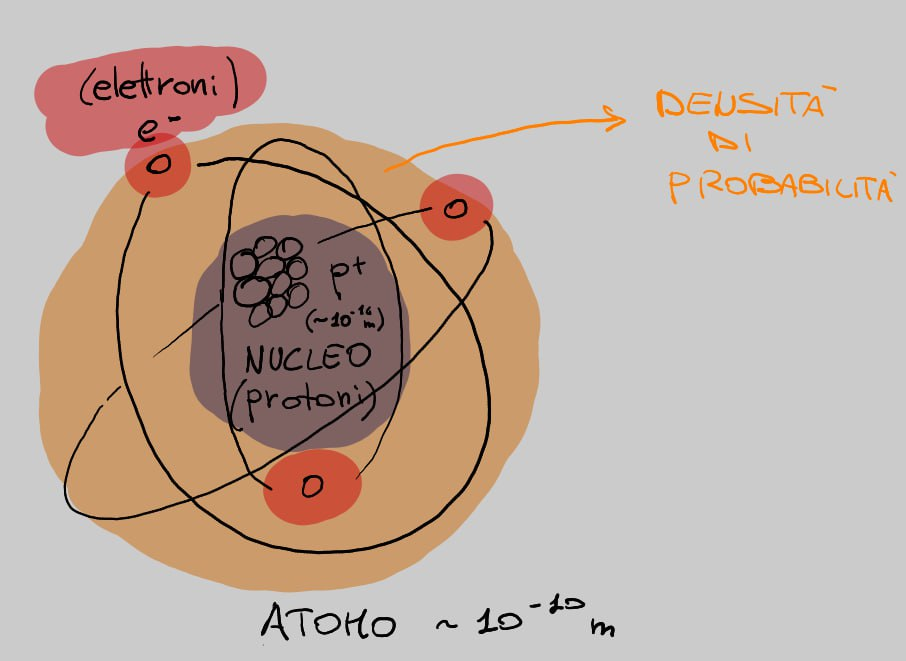
\includegraphics[scale=0.4]{atomo}
    \end{center}
    \begin{itemize}
        \item Gli \emph{elettroni} ($e^-$) sono particelle a \emph{carica negativa} e sono in uno stato legato con il nucleo.
        \item Il nucleo \`e formato da \emph{protoni}, particelle di carica positiva ($q^+$), e neutroni, particelle senza carica. 
        I protoni hanno una massa pari a 1836 volte quella di un elettrone.
    \end{itemize}
\end{multicols}

Si ha che $q_p^+ = | q_e^- |$, ovvero la carica del protone \`e uguale in modulo  quella dell'elettrone.

\section{Eletrizzazione}

Un oggetto pu\`o essere caricato elettricamente in tre modi: per strofinio, attraverso l'induzione elettrica
e con il contatto.

\subsection{Strofinio}

Supponiamo di avere un panno e una bacchetta, di qualsiasi materiale. Se strofiniamo il panno sulla bacchetta 
vi sar\`a uno spostamento di elettroni dalla bacchetta al panno, rendendo perci\`o la bacchetta carica elettricamente.

\begin{center}
    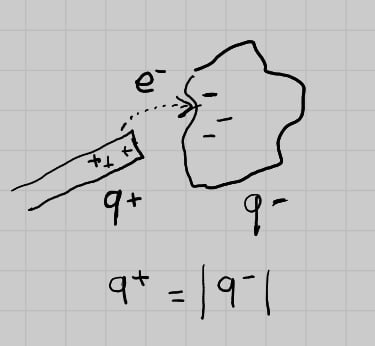
\includegraphics[scale=1]{strofinio}
\end{center}


\end{document}